	\section{Le parser}\label{sectionParser}
	Avant mon arrivée, le client et l'équipe avait conçu une grammaire de langage permettant de spécifier le fonctionnement du test, afin d'effectuer un scénario de stimulation ou une \textit{Expected Behavior} il faut respecter une syntaxe précise, dans le cas contraire une exception est levée.

	\subsection{La grammaire}\label{specParser}
	\subsubsection{Les scénarios de stimulations}
	Un \textit{precondstim} peut contenir des affectations, des \textit{check} et des actions débugger : 
	\begin{description}
		\item[Affectation] Une affectation s'effectue de la façon suivante : \texttt{Alias = valeur}, l'alias \texttt{Alias} possédera ensuite la valeur \texttt{valeur}.
		\item[Check] Cette action permet de vérifier qu'un alias possède bien la valeur espérée, à une tolérance prêt. Dans le cas contraire le bundle ne pourra pas être exécuté et une exception sera levée. Cela s'effectue ainsi : \texttt{CHECK(Alias = Valeur, TOLRES(tolerance))}, la tolerance étant facultative.
		\item[Actions débugger] Il est actuellement possible d'effectuer deux actions : démarrer le debugger, ou l'arrêter : \texttt{T32\_GO} et 
		\texttt{T32\_CPU\_STOP}.
	\end{description}

	Les scénarios de stimulations quant-à eux ont le même fonctionnement, la seule différence est qu'ils doivent être encadrés des balises \texttt{BEGIN SCENARIO nomScenario} et \texttt{END SCENARIO}.

	\subsubsection{Le fichier cnf}
	Comme nous l'avons expliqué, les tests sont spécifiés dans le fichier \textit{Walkthrough} qui est au format Excel, étant donné la difficulté d'éditer de longs texte dans la même cellule, il parait important de mettre les scénarios de stimulations dans un autre fichier : c'est l'utilité du fichier cnf, celui-ci contiendra des groupes d'actions à effectuer, spécifiés par un nom\footnote{Cela pourrait s'approcher du fonctionnement de sous-programmes} : le fichier Excel pourra ainsi ne contenir que le nom du groupe d'action, et de la place sera gagnée dans la cellule.

	La syntaxe du fichier est assez simple :
\begin{lstlisting}[caption=Exemple de fichier cnf, language=C]
// Section for group of parameters
SECTION SUB
	SUB_ECU_GO : {
		HIL_VB = 13;
 		HIL_KEY = 1;
		CHECK(HIL_KEY_OUT = 1);
		T32_GO;
	}

	SUB_ECU_OFF : {
		T32_CPU_STOP;
 		HIL_KEY = 0;
		HIL_VB = 0;
	}

	SUB_SCENARIO_VS_0_50_0 : {
		HIL_VS = 0;
		CHECK(HIL_VS_OUT = 0,  TOLRES(1)) ;
		HIL_VS = 0;
		CHECK(HIL_VS_OUT = 50,  TOLPER(1)) ;
		HIL_VS = 0;
		CHECK(HIL_VS_OUT = 0, TOLRES(1));
	}

END SUB
\end{lstlisting}
\begin{remarque}
Il y a une différence sémantique entre \texttt{TOLRES} et \texttt{TOLPER} : \texttt{TOLRES} est une tolérance en terme de valeur, alors que \texttt{TOLPER} est une tolérance en pourcentage. 
\end{remarque}
Un simple appel à \texttt{SUB\_ECU\_GO} dans le fichier Excel fera les actions nécessaires. Cette approche permet de gagner de la place comme indiqué, mais elle permet aussi de factoriser les tests !

	\subsubsection{Les expected Behavior}
Comme expliqué précédemment, les Expected Behavior sont des expressions permettant d'évaluer une trace, celles-ci ont une syntaxe proche d'un langage algorithmique : 
\begin{lstlisting}[caption=Exemple d'expected Behavior, language=Algo]
if tco > c1 then 
	EVAL(lv_cfa = 1)
else
	if(tco < c2) then 
		EVAL(lv_cfa = 0)
	else           
		EVAL(lv_cfa = PRE(lv_cfa))
	endif
endif
\end{lstlisting}
La grammaire est récursive, il est possible d'effectuer plusieurs \texttt{Eval} à la suite : ceux-ci doivent être séparés par un retour chariot.

Le mot clé \texttt{PRE}\footnote{Pour previous} permet de récupérer la valeur précédente de la variable en paramètre, l'instruction \texttt{lv\_cfa = PRE(lv\_cfa)} permet de vérifier que la variable n'a pas changée.

\subsubsection{Les alias locaux}
Une autre grammaire nécessaire est celle des alias locaux : les alias déclarés uniquement pour le test courant. Un certain nombre d'informations est nécessaire : le nom de l'alias, l'adresse, et les informations permettant de convertir celui-ci en valeur physique.

\begin{lstlisting}[caption=Exemple de définition d'alias local, language=Algo]
Alias_name = @HEXA;tailleOctet[8000...7FFFH]
\end{lstlisting}
L'alias aura une valeur hexadécimale, une taille en nombre d'octet, ainsi qu'une valeur de début et une valeur de fin afin de savoir les limites de définition de cette variable.

\subsubsection{Variables à enregistrer}
Il est possible de fournir des variables à enregistrer en plus de celle présente dans l'\textit{Expected Behavior} : cela permet d'avoir le contexte d'exécution, et de mieux comprendre la raison de l'échec d'un test. La définition de ces alias est très simple, ceux-ci doivent simplement être séparés par des virgules.

\begin{lstlisting}[caption=Exemple de définition d'alias à enregistrer, language=Algo]
FlSys_stFlLvl, C_FlSys_stFlLvl, LV_REQ_ES_AAS, LV_AAS_ACT
\end{lstlisting}

	\subsection{Implémentation du parser}
		\subsubsection{La grammaire : utilisation de Antlr}
		\begin{wrapfigure}{r}{3cm}
			
\includegraphics[width=3cm]{contents/images/antlr.jpg}
		\end{wrapfigure}
		J'étais en charge d'écrire le parser spécifié dans la section \ref{specParser}. Comme nous l'avons vu, celui-ci intègre beaucoup de grammaires différentes, notamment celle des \textit{Expected Behavior} qui est assez complexe. \\
		Une solution a été choisie afin d'optimiser au maximum le temps de développement et de limiter les erreurs : utilisation de Antlr\footnote{ANother Tool for Laguage Recognition}.

		Antlr est un framework libre de construction d'interpreteurs, il prend en entrée une grammaire, définissant notre langage à reconnaître et produit automatiquement le code Java permettant de reconnaître ce langage, ceci en parcourant l'arbre syntaxique. Il ne nous est donc plus nécessaire d'effectuer cette partie du travail, il faut simplement que nous effectuons les bonnes actions en fonction de notre emplacement dans l'arbre.

		Antlr à une syntaxe très simple pour définir une grammaire, il est nécessaire de déclarer tous nos mots clé tel que \texttt{if}, \texttt{check}, mais aussi les caractères utilisés dans le langage tel que \texttt{(, ), {; }} où simplement le retour chariot\footnote{Celui-ci correspondant à \texttt{\textbackslash n} ou \texttt{\textbackslash  n\textbackslash r} sous Windows}. Une fois que nos mots clés sont déclarés, il est possible de construire nos grammaires : pour cela, Antlr possède un outil de conception de grammaire, celui-ci a la particularité de construire le diagramme du langage en temps réel. Voici deux exemples de grammaires que j'ai rédigé :

		\paragraph{Grammaire du Check}~\\
\begin{lstlisting}[caption=Grammaire Check, numbers=none]
checkFunc : Check OBracket Alias Equals (Real|Integer) (Coma (tolres|tolper))? CBracket;
\end{lstlisting}
Dans la partie gauche de cette expression, nous avons le nom du \textit{token}, sur la partie droite sa définition. Les mots commençant par une majuscule sont des constante se rapportant à un caractère, le pipe \texttt{|} signifie un <<ou>>, et le point d'interrogation \texttt{?} signifie que l'expression le précédant est facultative, quant-au mots commençant par une minuscule, ce sont des mots se rapportant à la définition d'un autre \textit{token}, en l'occurrence ici à la définition de \texttt{tolres} et \texttt{tolper}. Ainsi le diagramme de cette expression est le suivant : 
\begin{figure}[H]
	\centering
	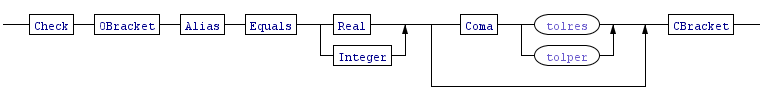
\includegraphics[width=18cm]{contents/images/check.png}
	\caption{Diagramme syntaxique du Check}
\end{figure}
		\paragraph{Grammaire de l'Expected Behavior}
		Une autre grammaire plus complexe, serait la grammaire des expected Behavior, disponible ci-dessous : 
\begin{lstlisting}[caption=Grammaire Check, numbers=none, language=C]
/* Expected Behavior 
 * Represents what we can meet in an expected Behavior Cell.
 */
ExpectedBehavior: NewLine?((
                  (If OBracket comparison CBracket Then NewLine? ExpectedBehavior NewLine?)
                  (Else NewLine? ExpectedBehavior NewLine? Endif))
                  | eval+)
                  NewLine?;
\end{lstlisting}
Le caractère plus \texttt{+} qui n'était pas présent précédemment représente la répétition de l'expression le précédent. Il est ainsi possible d'effectuer n'importe quel grammaire avec ces caractères de base. Comme nous pouvons le voir, la grammaire est récursive. Son diagramme syntaxique est présent figure \ref{fig:diagSynEB}.
\begin{figure}[H]
	\centering
		\hspace*{-40px}
	\includegraphics[width=20cm]{contents/images/ExpectedBehaviorGrammar.jpg}
	\caption{Diagramme syntaxique du Check}
	\label{fig:diagSynEB}
\end{figure}
\begin{remarque}
Le diagramme devrait contenir des \texttt{Newline} facultatifs au début et à la fin, ceux-ci ont été omis par soucis de lisibilités du diagramme en raison de sa largeur.
\end{remarque}

Une fois toutes les grammaires construites avec l'intégralités des n\oe{}uds de l'arbre d'expression, il suffit de générer les fichiers java, et de parcourir l'arbre d'expression.

	\subsubsection{La visite de l'arbre d'expression}
	Antlr propose plusieurs méthodes afin de reconnaître notre langage, nous avons choisis d'utiliser les \textit{visitors}. Le concept est assez simple : Nous devons hériter d'une classe généré par Antlr, qui est nommée WalkthroughBaseVisitor\footnote{Walkthrough étant le nom du fichier contenant la grammaire antlr}, c'est une classe générique nécessitant un type, notre grammaire retournera des \texttt{String}, mais dans le cas d'un parser d'expression, il peut être intéressant de retourner des \texttt{Numbers}.

	Cette classe contient une méthode par token présente dans la grammaire, il est possibles de les surcharger afin d'effectuer nos actions : chacune de ces méthodes ont pour convention de commencer par \texttt{visit} suivis par le nom du token. Ces méthodes sont appelés à chaque fois que nous passons dans ce n\oe{}ud de l'arbre. Celles-ci contiennent en paramètre le n\oe{}ud où l'on se trouve, il est donc possible de chercher des nœuds fils si-besoin, et ensuite d'appeler la suite de l'évaluation de l'arbre. 

	J'ai surchargé les méthodes qui était intéressantes ici tel que \texttt{visitCheckFunc(CheckFuncContext ctx)} présenté ci-dessous, le code est commenté afin d'aider à sa compréhension.
\begin{lstlisting}[language=Java, caption=Surcharge de \texttt{visitCheckFunc}]
	@Override
	public String visitCheckFunc(CheckFuncContext ctx) {
		String aliasName = ctx.getChild(2).toString(); // The alias name to check
		if(ctx.getChildCount() > 6) { // If tolerance is present
			// It's private method who call the generator, it will be explained after
			addCheckParam(aliasName, ctx.getChild(4).toString(), 
					(ctx.getChild(6).getChild(0).getText().equals("TOLRES") ? TolType.TOLRES : TolType.TOLPER), 
					ctx.getChild(6).getChild(2).getText());
		} else {
			addCheckParam(aliasName, ctx.getChild(4).toString());
		}
		// Generator too
		aliasReadableRequired.add(new AliasReadable(aliasName));

		return super.visitCheckFunc(ctx); // call next node of tree
	}
\end{lstlisting}
		\subsubsection{La gestion des exceptions}
\'Etant donné le temps d'exécution des tests\footnote{Environ une quinzaine d'heures}, il était nécessaire d'effectuer le maximum de vérification avant la phase d'exécution afin de ne pas avoir une erreur qui remonte au bout de plusieurs heures d'exécutions. 

Pour cela, nous avons utilisés plusieurs stratagèmes, tout d'abord l'utilisation d'un langage fortement typé tel que le Java, à l'opposé du Python utilisé sur la TA3, nous permet de générer du Java qui en cas d'erreur de type ne compilerait pas\footnote{Comme l'écriture sur un alias en lecture}, mais l'autre approche était l'utilisation des exceptions lors du parsing.

Une fois le parsing de l'intégralité des variables du \textit{Walkthrough} effectué, si au moins une ligne n'a pas pu être parsé, une exception est retourné contenant le message de toutes les erreurs trouvés durant ce parsing, toutes les lignes n'ayant pas obtenu d'erreur sont tout de même générés.

J'ai également mis en place un système de log avec \texttt{log4j} qui permet d'afficher proprement des messages de logs et de gérer la sévérité. Si une exception de parsing est renvoyée, celle-ci sera affichée dans la sortie standard, et dans le fichier de log.

Nous pouvons les dissocier en deux types d'exceptions : les erreurs de syntaxe et les erreurs d'Alias. 
\paragraph{Erreurs de syntaxe} Ces erreurs sont en partie gérer par Antlr, c'est purement syntaxique tel que l'oubli d'un caractère, cependant les erreurs Antlr n'étant pas clair, j'ai surchargé leurs méthodes d'affichage d'une part, afin d'avoir un affichage comme montré ci-dessous, mais j'ai également surchargé leurs gestionnaires afin de renvoyer une exception, ce qui n'était pas fait précédemment. L'envoie d'une exception permet de traiter le problème plus haut : c'est le \texttt{TestManager} qui la traitera.
\begin{lstlisting}[caption=Affichage d'une erreur de syntaxe, numbers=none]
line 34:10 mismatched input '0' expecting ';'
HIL_VB  0;
       ^
\end{lstlisting}


\paragraph{Erreurs d'alias} Ces erreurs sont des erreurs sémantiques au niveau des Alias, elles sont regroupées en 3 types différents : 
\begin{description}
	\item[Alias non connu] Cela signifie que l'alias n'est connu nul part, il ne pourra donc pas être résolu lors de l'execution des tests
	\item[Alias en lecture seule] L'utilisateur a essayé d'écrire sur un alias en lecture.
	\item[Alias en écriture seule] Il n'est pas possible de lire la valeur d'un alias en écriture.\\~
\end{description}

\begin{lstlisting}[caption=Affichage d'une erreur d'alias, numbers=none]
Error: Alias unknown [HL_VSd, Alias, Test]
Error: Alias not readable [HIL_VS, HIL_VB]
Error: Alias not writable [HIL_VS_OUT, HIL_VB_OUT]
\end{lstlisting}
		
